\newpage
\section{Diffusion Distance}

\begin{figure}[h]
 \centering
 \captionsetup{justification=centering,margin=2cm}
  \subfloat[]{
   \label{fig:d}
    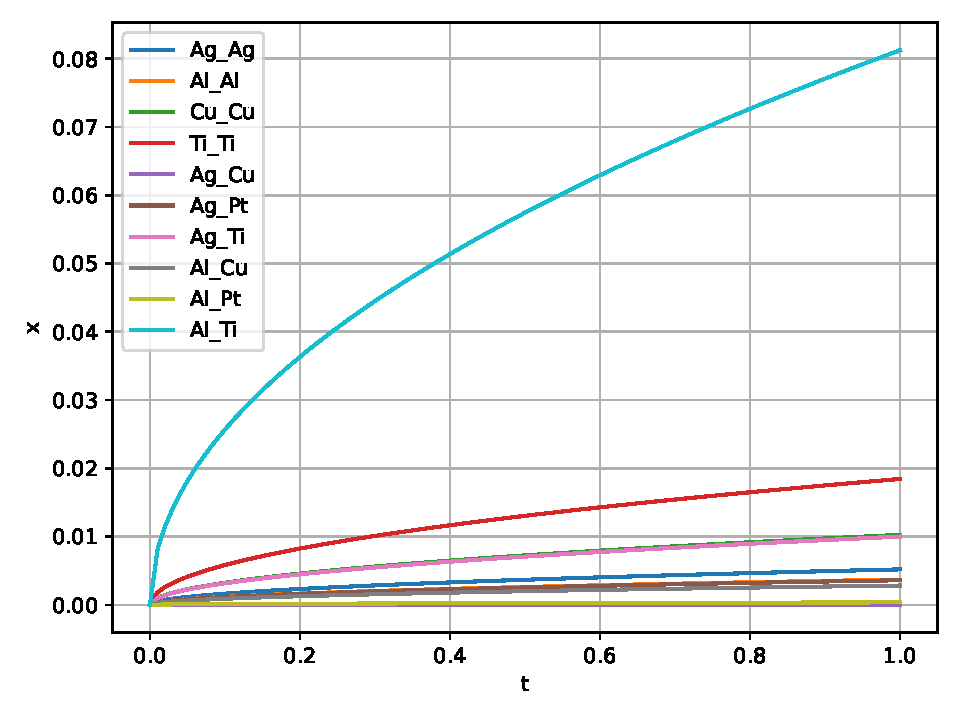
\includegraphics[width=0.5\textwidth]{graficas/x.pdf}}
  \subfloat[]{
   \label{fig:lnd}
    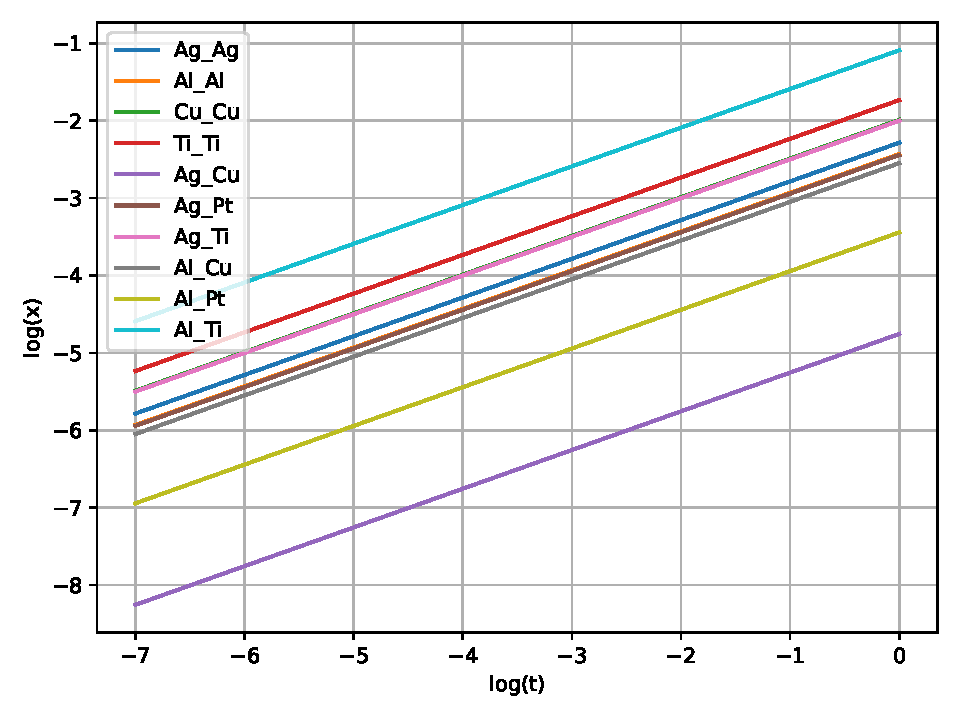
\includegraphics[width=0.5\textwidth]{graficas/log(x).pdf}}
 \caption{a) Diffusion coefficient $D$ ($m^2/s)$ as a function of temperature $T$ (K) and b) logarithm of the diffusion coefficient $ln(D)$ as a function of the inverse of temperature $1/T$ ($K^{-1}$). \\
 \textit{Source: Data from \citep{kakusan}, visualization by the author (code available at \citep{mygit}).}}
 \label{fig:diffusion}
\end{figure}


\subsection{Self-diffusion}

\begin{figure}[h]
 \centering
 \captionsetup{justification=centering,margin=2cm}
  \subfloat[]{
   \label{fig:}
    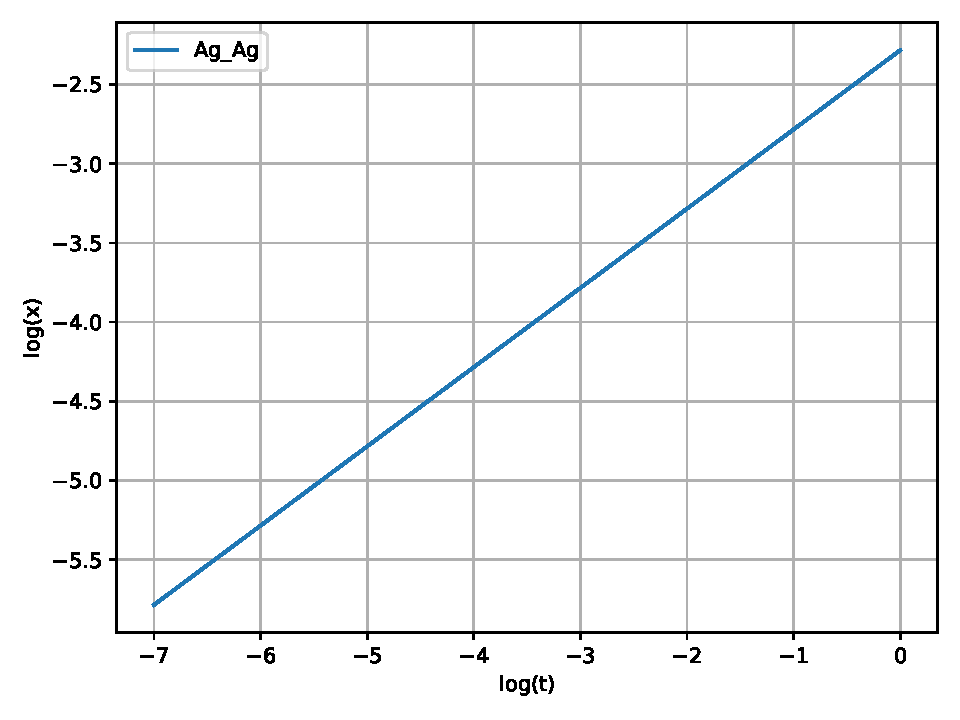
\includegraphics[width=0.5\textwidth]{graficas/Ag_Ag_log(x).pdf}}
  \subfloat[]{
   \label{fig:sigma4}
    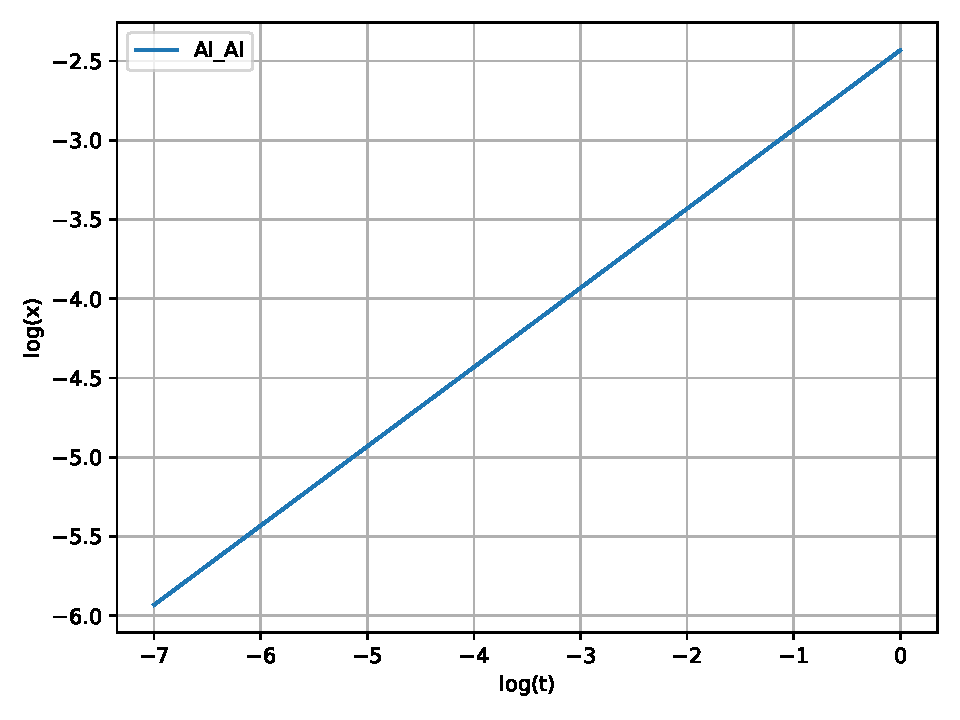
\includegraphics[width=0.5\textwidth]{graficas/Al_Al_log(x).pdf}} \\
  \subfloat[]{
   \label{fig:}
    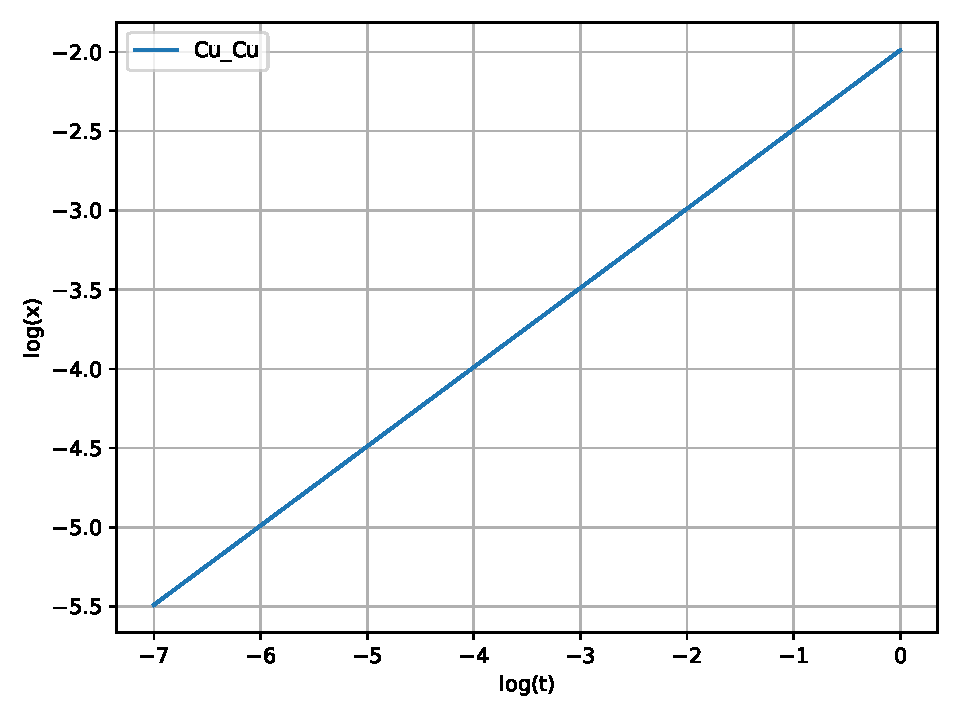
\includegraphics[width=0.5\textwidth]{graficas/Cu_Cu_log(x).pdf}}
  \subfloat[]{
   \label{fig:sigma4}
    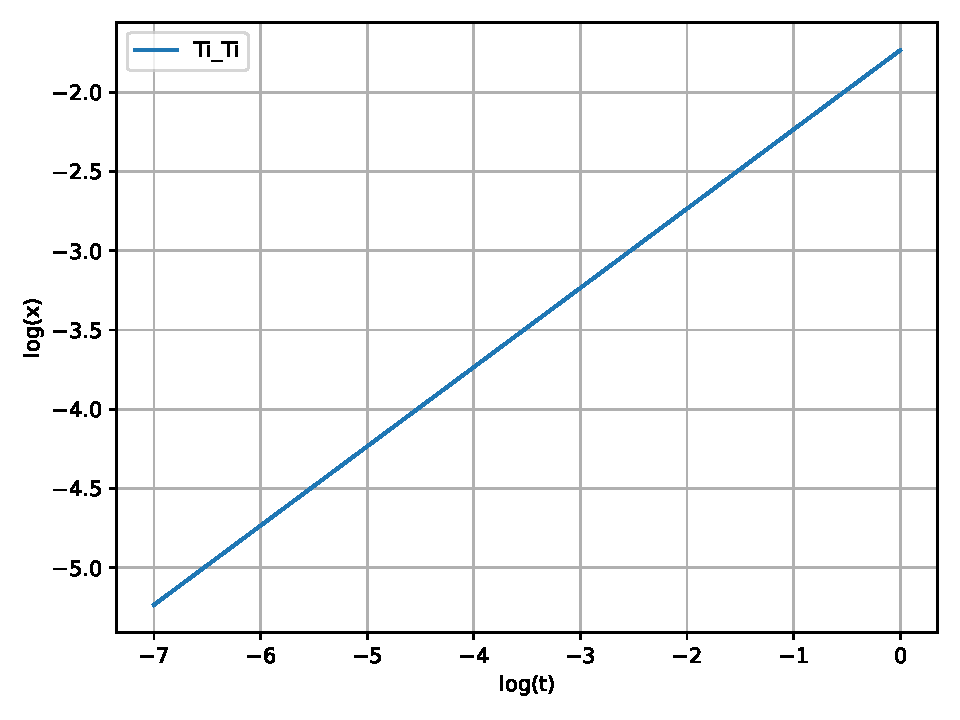
\includegraphics[width=0.5\textwidth]{graficas/Ti_Ti_log(x).pdf}}
 \caption{Logarithm of the diffusion coefficient for self-diffusing systems: a) silver, b) aluminum, c) copper and d) titanium.\\ 
 \textit{Source: Data from \citep{kakusan}, visualization by the author (code available at \citep{mygit}).}}
 \label{fig:selfdiff_lnd}
\end{figure}


\subsection{Solute diffusion}



(c) For the metals and solute atoms covered in question (a), assuming a sufficiently large sample size, graph the self-diffusion distance (logarithm) and the solute atom diffusion distance at room temperature against time (logarithm).
